\documentclass{article}
\usepackage[margin=1in]{geometry}
\usepackage{graphicx}

\graphicspath{{../screenshots/}}
\usepackage{xeCJK}

\usepackage{lipsum}
\setCJKmainfont{Noto Serif CJK TC}

\author{Andr\'es Ponce (0616110) \
\and
彭思安}
\title{Networks Systems Capstone Lab 1 Report}


\renewcommand{\familydefault}{\sfdefault}

\begin{document}
\maketitle
\section{Part 1}

\subsection{Flush all switch tables and take screenshots to show the switch tables of all
switches.}
\begin{figure}[h]
	\centering
	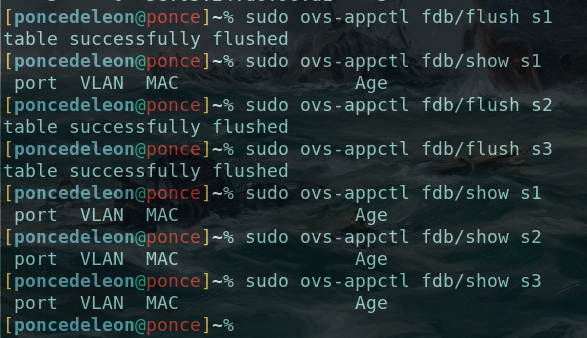
\includegraphics[scale=0.4]{flushSwitch.png}
	\caption{Flushing the routing tbales for the three switches, then showing their empty tables.}
\end{figure}

\subsection{How does \texttt{h4} know \texttt{h1}'s MAC address? Take screenshot on 
Wireshark to verify your answers.}
\begin{figure}[h]
		\centering
		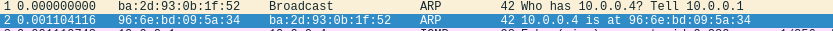
\includegraphics[scale=0.4]{ARP.png}
		\caption{\texttt{h1} sending an ARP message to determine the MAC address of
		\texttt{h4}.}
		\label{fig:Part1}
\end{figure}
Before the first \texttt{ping} command is sent, \texttt{h4} will receive an ARP 
broadcast message with a request from \texttt{h1}, for anybody with that IP address.
The sender (\texttt{h1}) determines the IP address of the receiver (\texttt{h4}) since before
the first \texttt{ping} request is sent.
\texttt{h4} then responds with its MAC address.

\subsection{How does \texttt{h1} know \texttt{h4}'s MAC address? Take screenshot on 
Wireshark to verify your answers.}

At the very beginning, \texttt{h1} will determine the IP address of the recipient and then send
an ARP broadcast message to all the other hosts on the local network. 
ARP is a link-layer protocol to determine the MAC address of another computer on the local network.
The destination will respond with its MAC addresss to the broadcast message.

\subsection{Why does the first ping have a longer delay?}
The first ping request-response cycle is slower due to the updating of the 
eouting table within each router.

\section{Part 2}
\subsection{Can \texttt{h1} ping \texttt{h4} successfully before enabling STP?}
The \texttt{ping} command cannot run effectively before we enable STP\@. 
STP is a protocol designed to construct a network topology without any switching loops.
These loops result from multiple redundant connections between different switches to improve
network resillience. 
However, before we enable STP on every switch in the network, we cannot know exactly how to send 
packets in a way that avoids these loops.

\subsection{Can \texttt{h1} ping \texttt{h4} successfully after STP is enabled?}
Yes, once we allow STP to operate on the current network topology, the
switches know where to route all the packets.

\subsection{Show \texttt{s1} MAC tables before and after STP is enabled and 
explain the differences.}
\begin{figure}[h]
	\centering
	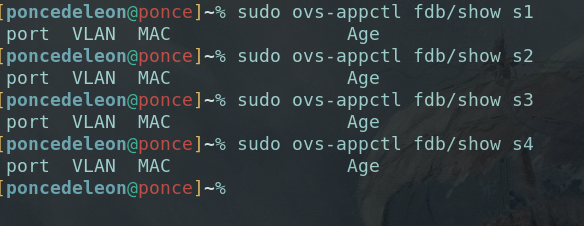
\includegraphics[scale=0.4]{NoSTPMAC.png}
	\caption{Routing tables for all the switches before enabling STP.}
\end{figure}

Before we run STP, the routing tables in all the switches are emtpy. 
Thus when we send information from \texttt{h1} to \texttt{h4}, our network still cannot
avoid switching loops.

\begin{figure}[h]
	\centering
	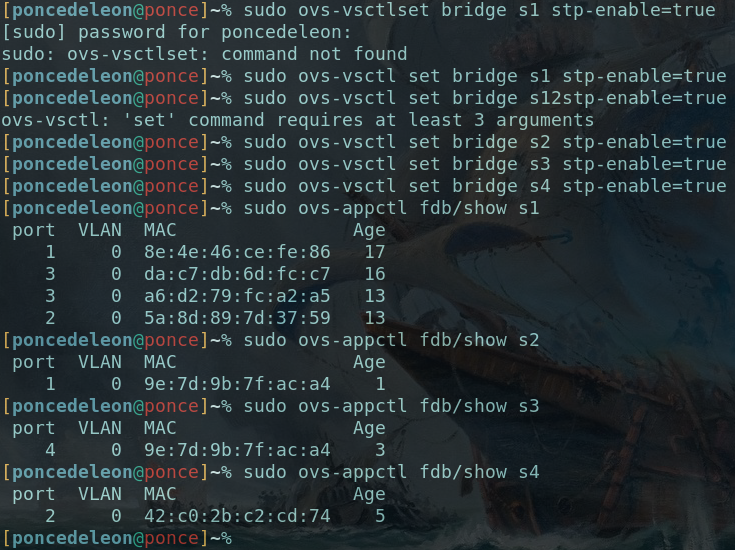
\includegraphics[scale=0.4]{STPMAC.png}
	\caption{Routing tables for all the switches after enabling STP.}
	\label{fig:STPRouting}
\end{figure}

After we enable STP, the routing tables can be built normally, and the request made to another
host on the same network.

The difference in these two tables can be seen from Figure~\ref{fig:STPRouting}, 
where after the \texttt{ping} message, where the routing table is filled in with 
the information of the MAC address for the hosts.

\subsection{What have you observed and learned from this lab?}
This lab allowed me to refresh on the different protocols active in the Link Layer. 
It also served as a reminder on mininet and how to create networks with given properties
in software.
After not having taken a networks course in more than one year, reintroducing even some of the most
fundamental ideas in local networks was useful for some of the topics covered later on in the course.

I had also forgotten the STP algorithm and its usefulness in redundant local networks.
The STP algorithm can help detect and avoid bridge loops in local networks via Ethernet.
The reason why there was no problem in running the network in the first problem was because the 
topology was much simpler, there was only one path from \texttt{s1} to \texttt{s3}.
Once we introduced the possibility of loops, a more sophisticated approach was 
required, thus we used STP to construct the routing tables at every switch.
\end{document}
